% ============================================================
%  \subsection{Site Map}
%  aBridgeAI — Capstone Report
%  Full per-route URL listing is documented in Appendix \ref{appendix:sitemap}.
% ============================================================

\subsection{Site Map}

The application is a single-page web client built with \textbf{Vite} and \textbf{TanStack Router}, served as a static bundle from a CDN and consuming the FastAPI backend over HTTPS. All authenticated routes are nested under a single \texttt{authenticatedRoute} parent that enforces a session check and an MFA gate before any child route is allowed to mount; deep-linked routes round-trip through \path|/login| with a \path|next| query parameter so users land back on the originally requested URL after authentication.

Figure~\ref{fig:sitemap} summarises the full route tree, organised by the five role groups exposed by the platform: \textit{Public}, \textit{Student}, \textit{Instructor}, \textit{Educational Manager}, and \textit{Administrator}. The complete per-route URL listing --- with page name, dynamic parameters, and purpose for each of the 59 routes --- is provided in Appendix~\ref{appendix:sitemap}.

\begin{figure}[H]
    \centering
    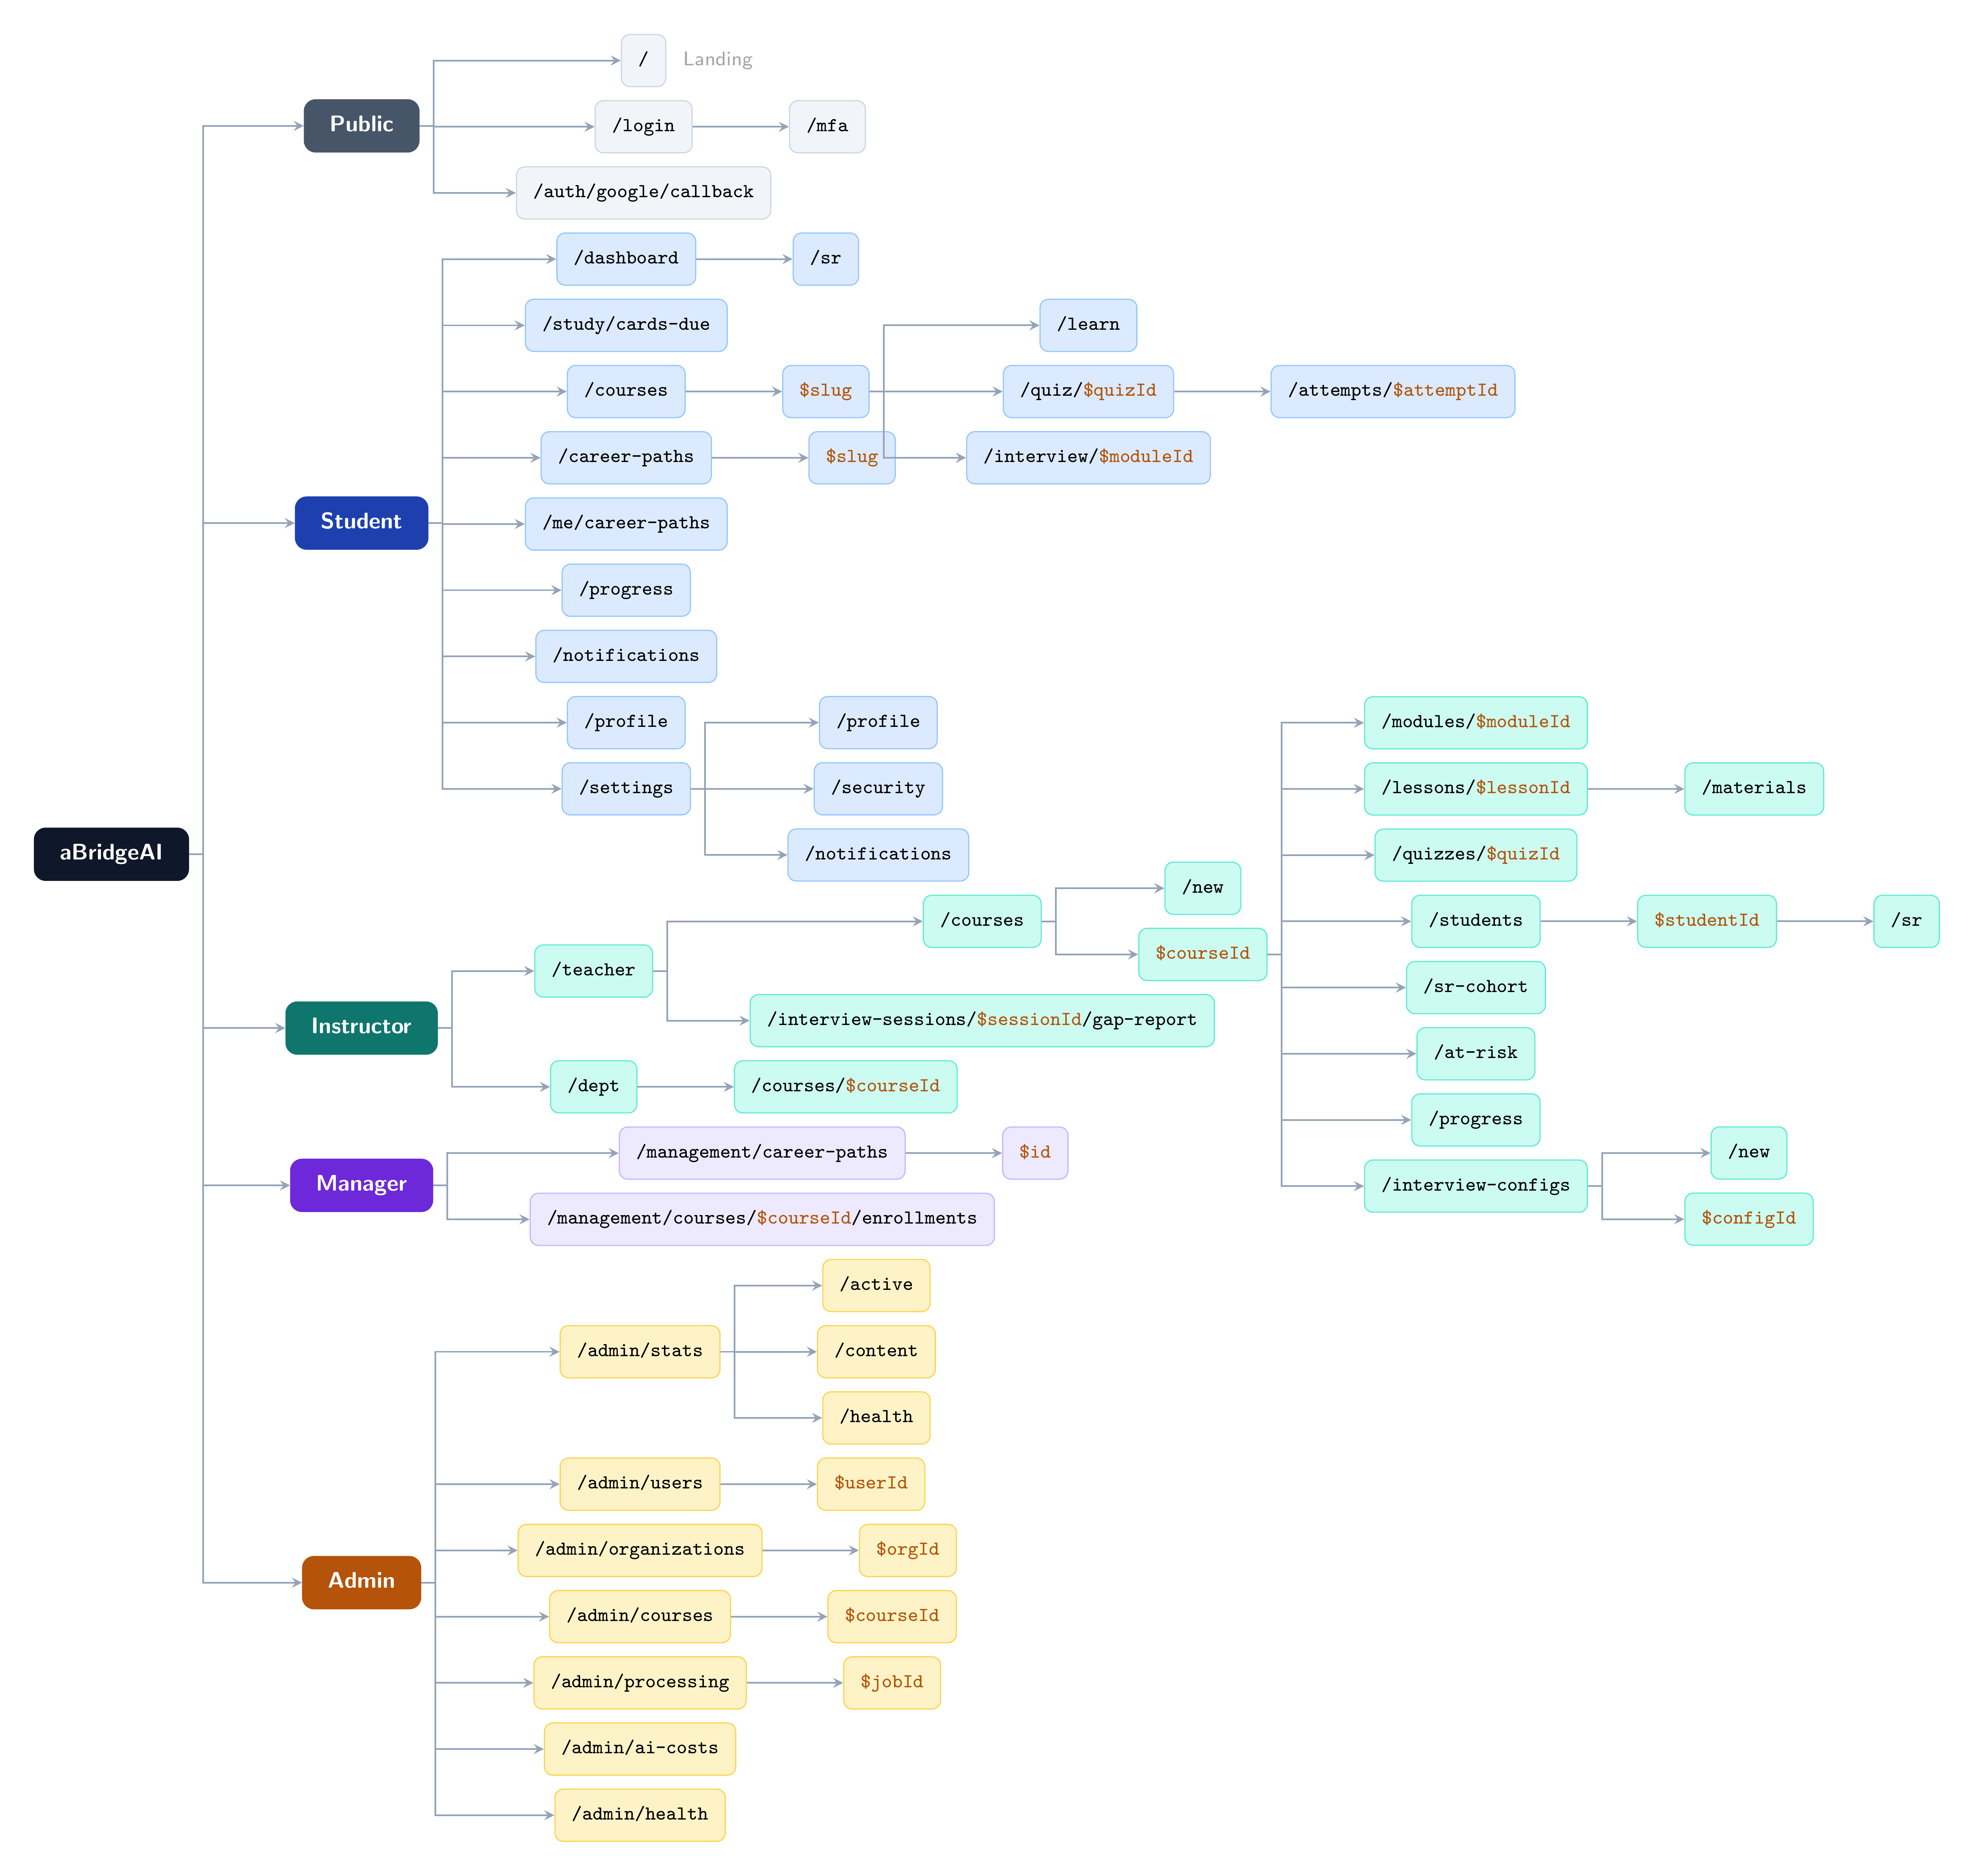
\includegraphics[width=\textwidth]{graphics/screenshots/sitemap_diagram.png}
    \caption{Application sitemap --- colour-coded by role group: grey (public), blue (student), teal (instructor), violet (educational manager), amber (administrator). Dynamic URL segments are highlighted in amber as \texttt{\$param}.}
    \label{fig:sitemap}
\end{figure}

The sitemap is intentionally flat within each role group: there are no role-specific subdomains, only path prefixes (\path|/teacher|, \path|/admin|, \path|/management|, \path|/dept|), so a single deployment serves every persona. Role differentiation is enforced by the \path|beforeLoad| guard on the parent route plus the role-specific \path|navItems| array driving the sidebar. This keeps the bundle small (one client-side router for the whole platform) and makes it cheap to add new role-scoped routes --- a new admin page is one new \path|createRoute| call that joins the \path|authenticatedRoute| children list.
